\section{Objektivität und technische Vermittlung: Technisierung der Wissenschaften}

\subsection{Einführung: Wissenschaft, Technik und Objektivität}

Die Vorlesung untersucht,
wie sich wissenschaftliche Objektivität historisch verändert hat
und welche Rolle technische Instrumente
in der modernen Wissensproduktion spielen.

Im Zentrum steht die Frage,
wie wissenschaftliche Erkenntnis entsteht,
wenn Beobachtung,
Messung und Darstellung zunehmend
durch technische Verfahren vermittelt werden.

Wissenschaft erscheint häufig als objektiv,
weil sie sich auf Daten,
Messinstrumente,
Modelle und standardisierte Verfahren stützt.

Die Vorlesung zeigt jedoch,
dass auch diese Formen von Objektivität
eine Geschichte haben.

Zentrale Leitfragen:

\begin{itemize}
\item Was bedeutet wissenschaftliche Objektivität?
\item Wie verändern technische Instrumente wissenschaftliche Erkenntnis?
\item Warum sind Daten nicht einfach selbsterklärend?
\item Wie entsteht Vertrauen in wissenschaftliche Verfahren?
\item Weshalb kann wissenschaftliche Unsicherheit politisch instrumentalisiert werden?
\end{itemize}

Objektivität ist daher nicht einfach gegeben,
sondern entsteht durch historische,
technische,
soziale und institutionelle Praktiken.

\subsection{Quellenkritik und historisches Argumentieren}

Zu Beginn der Sitzung wurde nochmals
auf die Quellenkritik zu Kasparov und Deep Blue eingegangen.

Für die Prüfung ist wichtig,
dass Quellenkritik als Fliesstext geschrieben wird.

Es sollen also ganze Sätze formuliert werden,
nicht nur Stichworte.

Dabei müssen nicht alle möglichen Fragen beantwortet werden.

Entscheidend sind diejenigen Fragen,
die für Analyse und Interpretation der Quelle relevant sind.

Eine Quelleninterpretation soll sich nicht primär
an der persönlichen Meinung
der schreibenden Person orientieren.

Stattdessen geht es darum,
auf Grundlage der Quelle zu argumentieren.

Die zentrale Frage lautet also nicht:

Was denke ich selbst über Mensch und Maschine?

Sondern:

Wie lässt sich historisch erklären,
weshalb eine Quelle bestimmte Vorstellungen
über das Mensch-Maschinen-Verhältnis ausdrückt?

Wichtig ist daher eine stringente Argumentation.

Die eigene Interpretation muss begründet werden,
indem gezeigt wird,
wie sie aus der Quelle abgeleitet wird.

\subsection{Kasparov vs. Deep Blue als Beispiel der Quellenkritik}

Am Beispiel eines Zeit-Artikels
zu Kasparov und Deep Blue wurde gezeigt,
wie eine solche Quellenkritik aussehen kann.

Die Zeit ist eine liberale deutsche Wochenzeitung.

Der Artikel richtete sich nicht an Fachleute,
sondern an eine breite Leserschaft.

Technische Vorkenntnisse wurden nicht vorausgesetzt.

Der Artikel entstand zwischen dem ersten
und dem zweiten Aufeinandertreffen
von Garri Kasparov und Deep Blue.

Zu diesem Zeitpunkt war noch nicht bekannt,
dass Deep Blue Kasparov 1997 schlagen würde.

Der Artikel kündigte das zweite Spiel an
und blickte zugleich auf das erste zurück.

Auffällig ist,
dass Deep Blue einerseits personifiziert wird.

Es wird etwa von seinem „zweiten Leben“
oder von einer Software mit mehr „Gefühl“ gesprochen.

Andererseits wird seine technische Besonderheit
teilweise relativiert.

Es wird darauf hingewiesen,
dass es bereits andere Schachcomputer gebe,
die anders funktionierten
und in gewisser Weise moderner seien.

Der Artikel stellt also keine einfache Überlegenheit
der Maschine gegenüber dem Menschen fest.

Vielmehr erscheint Deep Blue
als Übergangsfigur einer älteren KI-Entwicklung,
während sich die KI-Forschung Ende der 1990er Jahre
bereits in andere Richtungen bewegte.

\subsection{„A Frank Statement to Cigarette Smokers“, 1954}

Ein zentrales Beispiel der Vorlesung
ist die Medienkampagne der US-amerikanischen Tabakindustrie
aus dem Jahr 1954.

Unter dem Titel
„A Frank Statement to Cigarette Smokers“
wandte sich die Tabakindustrie
an die Öffentlichkeit.

Hintergrund war,
dass wissenschaftliche Studien
seit dem frühen 20. Jahrhundert
auf die gesundheitlichen Gefahren des Rauchens hinwiesen.

Ab den 1950er Jahren nahm die Zahl der Todesfälle zu,
die mit Lungenerkrankungen in Verbindung gebracht wurden.

In den USA und anderen westlichen Staaten
begann man deshalb,
politische Regulierungen auszuarbeiten.

Dagegen wehrte sich die Tabakindustrie.

Die Kampagne stellte die wissenschaftlichen Arbeiten
nicht offen als unwissenschaftlich dar.

Stattdessen wurde behauptet,
dass die Beweislage noch nicht eindeutig genug sei.

Die Tabakindustrie argumentierte unter anderem:

\begin{itemize}
\item Medizinische Forschungen hätten auf viele mögliche Ursachen von Lungenkrebs hingewiesen.
\item Unter Fachleuten herrsche keine Einigkeit über die eigentliche Ursache.
\item Es gebe keinen Beweis dafür, dass Zigarettenrauchen eine Ursache sei.
\item Statistiken könnten ebenso gut andere Aspekte des modernen Lebens betreffen.
\end{itemize}

Damit wurde nicht die Wissenschaft als solche angegriffen.

Vielmehr wurden Unsicherheiten der wissenschaftlichen Beweisführung betont.

Ziel war es,
Zweifel zu säen.

\begin{center}
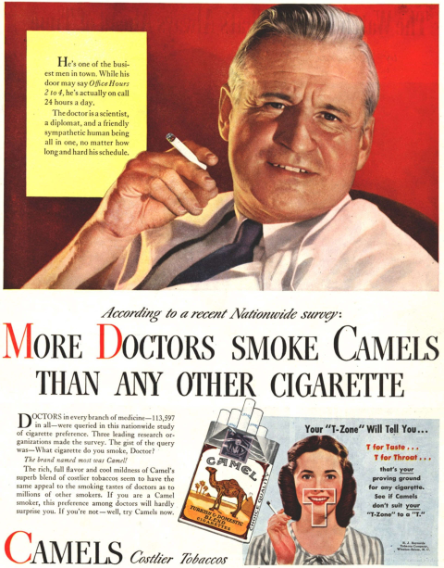
\includegraphics[width=0.65\linewidth]{images/frank_statement_cigarette_smokers.png}
\end{center}

\subsection{Strategische Unsicherheit und die Tabakindustrie}

In den folgenden Jahren
wurden ähnliche Kampagnen wiederholt durchgeführt.

Die Tabakindustrie stellte sich dabei nicht
grundsätzlich gegen Wissenschaft.

Sie bewegte sich vielmehr innerhalb
einer wissenschaftlichen Logik.

Behauptet wurde,
dass es noch keinen stichhaltigen Beweis
für den Zusammenhang zwischen Rauchen
und Lungenerkrankungen gebe.

Gleichzeitig investierte die Tabakindustrie
selbst in wissenschaftliche Forschung.

Diese Forschung sollte zeigen,
dass ein Zusammenhang nicht eindeutig bewiesen werden könne.

In den 1970er Jahren beauftragte
die R.J. Reynolds Tobacco Company
beispielsweise den renommierten Physiker Fred Seitz.

Seitz war ehemaliger Präsident
der US National Academy of Sciences.

Er trat nicht als Wissenschaftsskeptiker auf.

Stattdessen erklärte er,
warum die vorhandenen Forschungsergebnisse
noch nicht ausreichten,
um klare Aussagen zu machen
oder politische Regulierungen zu begründen.

Daran zeigt sich eine wichtige Strategie:

Wissenschaftliche Unsicherheit wurde nicht beseitigt,
sondern gezielt produziert und verstärkt.

\subsection{Merchants of Doubt}

Eine ähnliche Strategie lässt sich
in den Debatten um das Ozonloch beobachten.

In den 1970er und 1980er Jahren
waren Wissenschaft und Politik
zunächst vorsichtig mit ihren Interpretationen.

Die Atmosphärenforschung war komplex,
die Datenlage begrenzt
und viele Fragen waren offen.

Diese Form von Unsicherheit
gehört grundsätzlich zur normalen wissenschaftlichen Praxis.

Sie ist sogar wichtig
für wissenschaftliche Glaubwürdigkeit,
weil Wissenschaft ihre eigenen Grenzen
und Unsicherheiten reflektieren muss.

Gleichzeitig wurden Umweltpolitik
und Regulierung ab den 1970er Jahren
zunehmend denkbar.

Deshalb traten Industrievertreter
und verbündete Wissenschaftlerinnen und Wissenschaftler
auf den Plan.

Besonders wichtig war dabei DuPont,
ein grosser Produzent von Fluorchlorkohlenwasserstoffen.

Diese Stoffe wurden unter anderem
als Treibgase,
Kältemittel und Lösemittel verwendet.

Industrievertreter zweifelten Messverfahren,
Modelle und Interpretationen an.

Sie forderten,
dass vor politischen Regulierungen
mehr Beweise geliefert werden müssten.

Auch hier wurde wissenschaftliche Unsicherheit
politisch genutzt.

\subsection{Die Entdeckung des Ozonlochs}

Im Jahr 1985 stellten britische Forscherinnen und Forscher
einen drastischen Rückgang der Ozonkonzentration
über der Antarktis fest.

Sie konnten den Zusammenhang
zwischen bestimmten Emissionen
und dem Ozonabbau nachweisen.

Diese Entdeckung führte später
zu weltweiten politischen Massnahmen.

Die Zweifel am Bestehen des Ozonlochs
verschwanden jedoch nicht sofort.

Trotzdem wurden auf politischer Ebene
verschiedene Massnahmen zur Reduktion
ozonschädigender Stoffe ergriffen.

Das Beispiel zeigt,
dass wissenschaftliche Erkenntnis
nicht automatisch und unmittelbar
zu politischem Handeln führt.

Zwischen Messung,
Interpretation,
Anerkennung und Regulierung
liegen gesellschaftliche und politische Aushandlungsprozesse.

\begin{center}
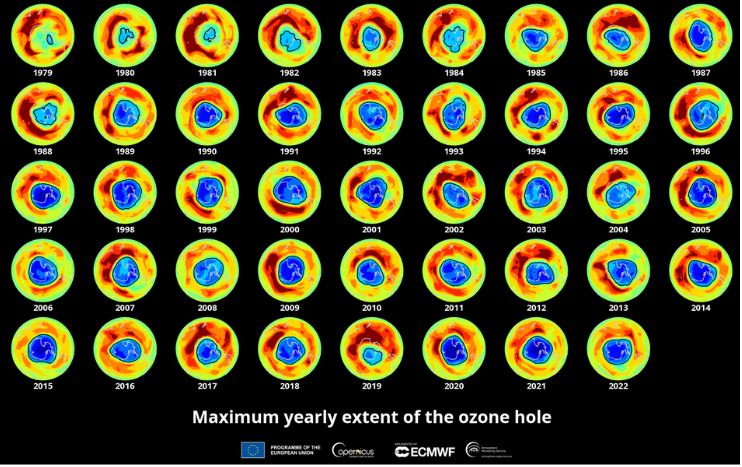
\includegraphics[width=0.75\linewidth]{images/ozonloch_1985.png}
\end{center}

\subsection{Objektivität und technische Vermittlung}

Besonders interessant ist,
dass die Satellitendaten,
mit denen das Ozonloch nachgewiesen werden konnte,
bereits früher vorhanden waren.

Sie wurden jedoch zunächst
als Ausreisser interpretiert
und aus den Berechnungen ausgeschlossen.

Die Werte erschienen zu extrem
und passten nicht in das bestehende Wissenssystem.

Sie wurden deshalb als Messfehler behandelt.

Das bedeutet:

Auch diejenigen,
die einen begründeten Verdacht
für die Existenz des Ozonlochs hatten,
vertrauten ihren Daten nicht blind.

Daten sprechen nicht einfach für sich selbst.

Sie müssen erhoben,
gefiltert,
korrigiert,
modelliert
und interpretiert werden.

Technische Messinstrumente liefern daher
keine unmittelbare Wahrheit.

Sie vermitteln zwischen Welt und Darstellung.

\subsection{Daten, Modelle und Interpretation}

Die Daten zum Ozonloch wurden nicht abgelehnt,
weil sie unwissenschaftlich gewesen wären.

Sie passten nicht
zu den vorhandenen Modellen
und Wissenssystemen.

Gerade bei komplexen Messinstrumenten
wie Satelliten ist dies besonders wichtig.

Satellitendaten brauchen Korrekturen,
Filter und Modelle.

Erst dadurch werden sie
zu wissenschaftlich nutzbaren Daten.

Daten sind also interpretationsbedürftig.

Wie sie erhoben,
bearbeitet
und als zuverlässig eingestuft werden,
ist nicht einfach gegeben.

Eine lückenlose Beweisführung
beruht daher immer auch
auf begründeten Annahmen.

Damit stellt sich die Frage,
was dies für den Objektivitätsanspruch
der Wissenschaft bedeutet.

\subsection{Die Geschichte des Objektivitätsanspruchs}

Die Vorlesung zeigt,
dass auch wissenschaftliche Objektivität
eine Geschichte hat.

Vor dem 19. Jahrhundert
stand häufig das Ideal der Naturwahrheit im Zentrum.

Gesucht wurde nicht unbedingt
die exakte Wiedergabe jedes einzelnen Details.

Stattdessen ging es darum,
das Wesentliche,
Typische,
Regelhafte oder Ideale der Natur zu erfassen.

Das Zufällige wurde zugunsten
eines Ideals korrigiert.

Ziel war es,
ein „inneres Gesetz“ der Natur zu erkennen.

Erkenntnis entstand durch geschultes Urteil.

Erfahrung,
Bildung
und Urteilskraft der Forschenden
galten als entscheidend.

Subjektivität wurde hier nicht als Fehler angesehen,
sondern als Kompetenz.

\subsection{Mit geschultem Urteil zur Naturwahrheit}

Beispiele für diese Form der Naturwahrheit
sind Carl von Linnés Taxonomie
und Robert Hookes \emph{Micrographia}.

Linnés Natursystem von 1758
ordnete Lebewesen nach systematischen Kriterien.

Dabei ging es darum,
Regelmässigkeiten und Ordnungen
in der Natur sichtbar zu machen.

Robert Hookes \emph{Micrographia} von 1665
zeigte mikroskopische Darstellungen,
etwa die berühmte Zeichnung eines Flohs.

Solche Darstellungen waren nicht einfach
mechanische Abbilder.

Sie beruhten auf Beobachtung,
Auswahl,
Zeichnung
und Urteil.

Wissenschaftliche Darstellung bedeutete,
das Gesehene so aufzubereiten,
dass sein wesentliches Merkmal
erkennbar wurde.

\begin{center}

\includegraphics[width=0.9\linewidth]{images/naturwahrheit_linne_hooke.png}
\end{center}

\subsection{Mechanische Objektivität}

Seit dem Ende des 19. Jahrhunderts
veränderte sich dieses Ideal.

Subjektivität wurde zunehmend
als unwissenschaftlich betrachtet.

Forschende sollten sich
so weit wie möglich zurücknehmen.

Wissenschaftliche Experimente wurden wichtiger,
und damit auch technische Instrumente.

Besonders neue Bild-
und Aufzeichnungsverfahren
galten als Mittel der Objektivierung.

Dazu gehörten:

\begin{itemize}
\item Photographie
\item Kymographen
\item automatische Aufzeichnungsgeräte
\item Bewegungsstudien
\item Messapparate
\end{itemize}

Individuelles Urteil
und subjektive Wahrnehmung
wurden durch technische Instrumente
in Frage gestellt.

Technik sollte das „Sehen“ übernehmen
und möglichst rohe Daten produzieren.

Statt idealisierender Darstellungen
sollten technische Aufzeichnungen
die Natur scheinbar unmittelbar festhalten.

\subsection{Technische Aufzeichnung und Objektivierung}

Beispiele für mechanische Objektivität
sind die Bewegungsstudien
von Eadweard Muybridge aus dem Jahr 1887
und die automatische Aufzeichnung
eines Bebens in Wien 1908.

Muybridges Fotografien zerlegten Bewegungen
in einzelne Bildsequenzen.

Dadurch konnten Bewegungsabläufe
technisch sichtbar gemacht werden,
die dem menschlichen Auge
in dieser Form nicht zugänglich waren.

Auch die automatische Aufzeichnung
eines Bebens zeigt,
wie technische Instrumente
als objektive Zeugen verstanden wurden.

Nicht mehr das geschulte Auge
der Forschenden sollte entscheiden,
sondern die Maschine sollte registrieren.

Damit entstand ein neues Ideal:

Objektiv ist,
was möglichst unabhängig
vom subjektiven Urteil
der Forschenden aufgezeichnet wird.

\begin{center}
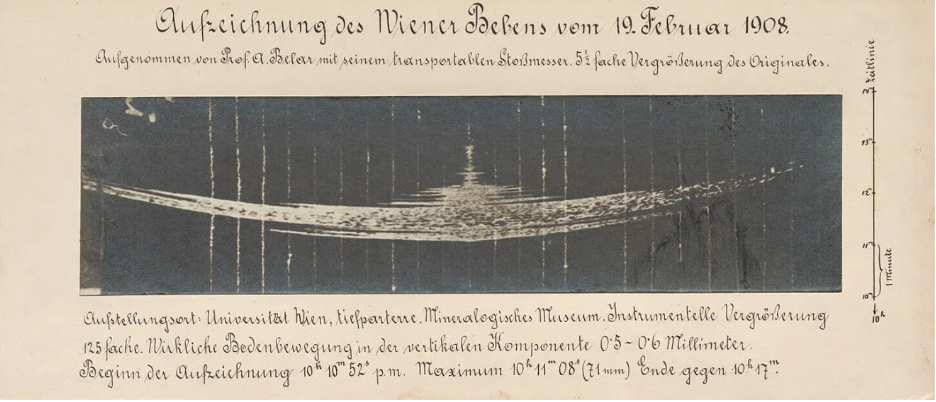
\includegraphics[width=0.9\linewidth]{images/mechanische_objektivitaet.png}
\end{center}

\subsection{Strukturelle Objektivität}

Im Verlauf des 20. Jahrhunderts
entwickelte sich zusätzlich
das Ideal der strukturellen Objektivität.

Diese löste die mechanische Objektivität
nicht einfach ab,
sondern entstand parallel dazu.

Sie erweiterte,
was als objektive wissenschaftliche Praxis galt.

In vielen Bereichen
wurde reines Aufzeichnen unpraktisch.

Besonders in der Atomphysik,
Quantenmechanik
oder Klimaforschung
sind die untersuchten Gegenstände
nicht mehr direkt beobachtbar.

Zudem erzeugen technische Messsysteme
riesige Datenmengen.

Deshalb wurden statistische Modelle,
mathematische Formeln,
formale Strukturen
und Simulationen zentral.

Forschende sollen sich dabei
in Regeln und Verfahren
wissenschaftlicher Praxis einfügen.

Sie treten hinter formale Systeme zurück,
bleiben aber dennoch Teil der Wissensproduktion.

\subsection{Modelle, Simulationen und wissenschaftliche Praxis}

Strukturelle Objektivität bedeutet nicht,
dass Forschende verschwinden.

Sie entscheiden weiterhin,
welche Modelle,
Daten,
Verfahren
und Annahmen verwendet werden.

Diese Entscheidungen müssen jedoch
innerhalb bestehender Wissenssysteme
begründet werden.

Objektivität entsteht also
durch nachvollziehbare Verfahren,
Standardisierung,
Dokumentation
und methodische Begründung.

Ein Beispiel dafür sind Klimamodelle.

Sie beruhen nicht auf einfacher Beobachtung,
sondern auf komplexen Simulationen.

Die in der Vorlesung gezeigte Simulation
mit historischen CO2-Emissionen
und einem angenommenen Emissionsstopp
am 1. Januar 2021
zeigt,
wie wissenschaftliche Erkenntnis
durch formale Modelle erzeugt wird.

Solche Modelle sind nicht einfach Bilder der Wirklichkeit.

Sie sind strukturierte,
technisch vermittelte Darstellungen,
die auf Annahmen,
Daten und Berechnungen beruhen.

\begin{center}
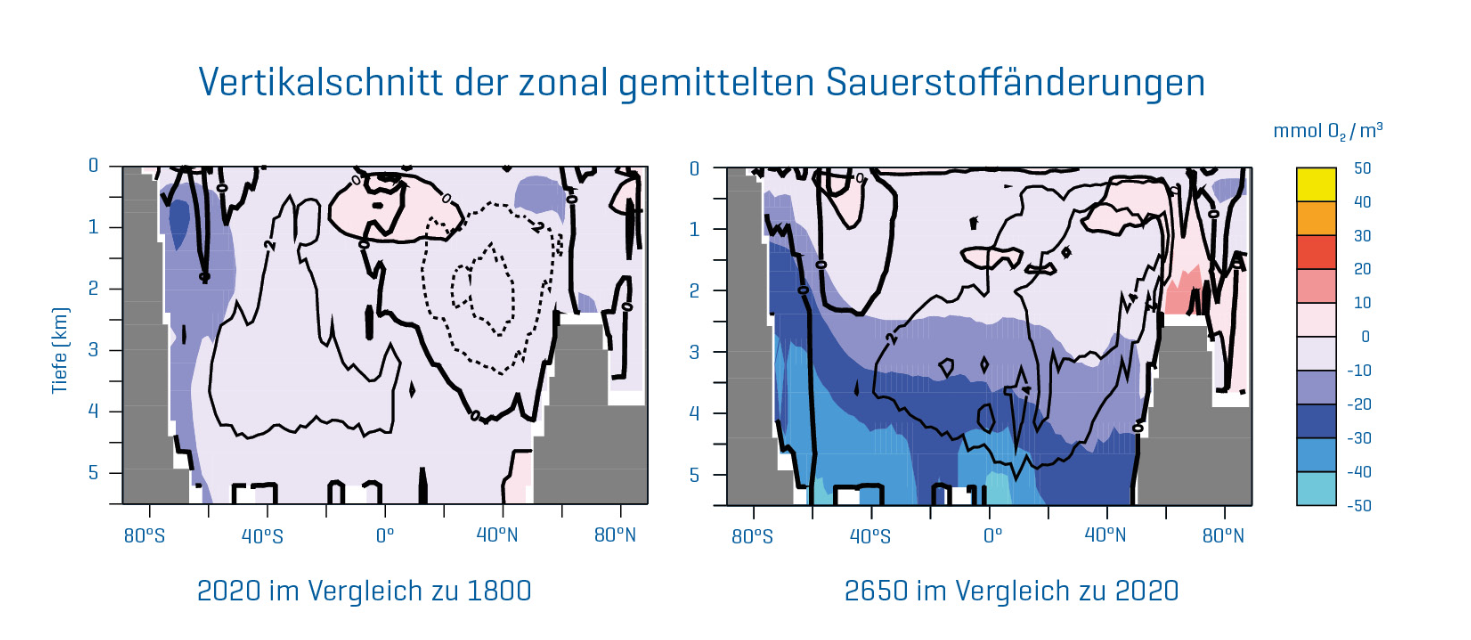
\includegraphics[width=0.9\linewidth]{images/strukturelle_objektivitaet_klimamodell.png}
\end{center}

\subsection{Glaubwürdigkeit und Technik}

Wie technische Instrumente
in der wissenschaftlichen Praxis eingesetzt werden,
stand historisch nicht einfach fest.

Innerhalb wissenschaftlicher Disziplinen
mussten sich stabile Praktiken herausbilden.

Diese Praktiken legten fest,
welche technischen Verfahren
als zuverlässig gelten konnten.

Dafür waren besonders wichtig:

\begin{itemize}
\item Standardisierung
\item Dokumentation
\item methodische Begründung
\item Wiederholbarkeit
\item disziplinäre Aushandlung
\end{itemize}

Vertrauen in technische Verfahren
entsteht also nicht automatisch.

Es ist Ergebnis historischer Aushandlungsprozesse.

Ein Messinstrument ist nicht allein deshalb glaubwürdig,
weil es technisch ist.

Es wird glaubwürdig,
wenn seine Anwendung stabilisiert,
dokumentiert
und innerhalb einer wissenschaftlichen Gemeinschaft
anerkannt wird.

\subsection{Angreifbarkeit wissenschaftlicher Objektivität}

Die Stabilisierung wissenschaftlicher Praktiken
ist nie völlig abgeschlossen.

Zudem ist sie von aussen
oft schwer nachvollziehbar.

Für Nicht-Fachleute ist es schwierig zu beurteilen,
ob ein Verfahren richtig oder falsch angewendet wurde
und welche epistemische Autorität es besitzt.

Das macht wissenschaftliche Objektivität
prinzipiell angreifbar.

Technische Vermittlung erzeugt immer eine Differenz
zwischen Welt und Darstellung,
zwischen Messung und Interpretation.

Diese Differenz kann in Zweifel gezogen werden.

Genau hier setzen Strategien
strategischer Unsicherheit an.

Die Tabakindustrie
und die Skeptiker des Ozonlochs
griffen nicht unbedingt Wissenschaft als Ganzes an.

Sie nutzten vielmehr die Tatsache,
dass wissenschaftliche Erkenntnis
immer technisch vermittelt,
modelliert
und begründungsbedürftig ist.

\subsection{Politische Dimension moderner Wissensproduktion}

Strategische Unsicherheit verweist
auf die politische Dimension
moderner und postmoderner Wissensproduktion.

Wissenschaftliche Unsicherheit
ist an sich nichts Unwissenschaftliches.

Sie gehört zur Wissenschaft.

Problematisch wird sie,
wenn Unsicherheit gezielt erzeugt,
übertrieben
oder politisch instrumentalisiert wird,
um Regulierung zu verhindern.

Die Beispiele der Tabakindustrie
und der Ozonloch-Debatte zeigen,
dass wissenschaftliche Objektivität
in politischen Konflikten
eine zentrale Rolle spielt.

Wer bestimmen kann,
was als bewiesen,
unsicher
oder noch nicht ausreichend geklärt gilt,
kann politische Entscheidungen beeinflussen.

Technik,
Wissenschaft
und Politik sind daher eng miteinander verbunden.

\subsection{Zentrale Erkenntnisse}

Die Vorlesung zeigt,
dass wissenschaftliche Objektivität
nicht zeitlos und unveränderlich ist.

Sie hat sich historisch gewandelt
und ist eng mit technischen Verfahren
der Beobachtung,
Messung,
Aufzeichnung
und Modellierung verbunden.

Zentrale Erkenntnisse sind:

\begin{itemize}
\item Objektivität ist eine historische wissenschaftliche Tugend.
\item Vor dem 19. Jahrhundert galt geschultes Urteil als zentrale wissenschaftliche Kompetenz.
\item Seit dem späten 19. Jahrhundert wurde mechanische Objektivität wichtiger.
\item Technische Instrumente sollten subjektives Urteil zurückdrängen.
\item Im 20. Jahrhundert gewannen Modelle, Simulationen und formale Verfahren an Bedeutung.
\item Daten sind nicht selbsterklärend, sondern müssen interpretiert und in Wissenssysteme eingeordnet werden.
\item Wissenschaftliche Unsicherheit kann politisch instrumentalisiert werden.
\end{itemize}

Die zentrale These lautet:

Technische Vermittlung macht Wissenschaft nicht weniger objektiv.

Sie zeigt aber,
dass Objektivität nicht einfach aus Daten entsteht.

Objektivität beruht auf Verfahren,
Instrumenten,
Modellen,
Standards,
Dokumentation
und begründeten Annahmen.

Gerade deshalb ist Wissenschaft glaubwürdig,
aber zugleich auch angreifbar.
